% Task 3: two contracts, one fingerprint. The matching variants are not shown.
\documentclass[12pt,tikz,border=6pt]{standalone}
% Shared preamble of the task figures of Lecture 7. The colours are the colour roles of the slides
% (main.tex) and of the passwords simulator:
%   Alice sIndigo, Mallory sPink, message / document / password sViolet, salt sAmber,
%   Bob / the server / the notary sTeal, digest sBrown; mechanisms dark; the unknown: orange dashed.
\usepackage{lmodern}
\usepackage[T1]{fontenc}
\renewcommand{\familydefault}{\sfdefault}
\usepackage{amsmath,amssymb}
\usepackage{xcolor}
\usepackage{fontawesome5}
\usetikzlibrary{arrows.meta, calc, positioning, fit, decorations.pathreplacing, backgrounds}

\definecolor{DeepBlue}{HTML}{283593}
\definecolor{AccentOrange}{HTML}{EB5A14}
\definecolor{nInk}{HTML}{37474F}
\definecolor{nLine}{HTML}{90A4AE}
\definecolor{nLight}{HTML}{CFD8DC}
\definecolor{nFill}{HTML}{ECEFF1}
\definecolor{aExec}{HTML}{43A047}
\definecolor{aWrite}{HTML}{E53935}
\definecolor{sIndigo}{HTML}{5C6BC0}
\definecolor{sPink}{HTML}{EC407A}
\definecolor{sViolet}{HTML}{7E57C2}
\definecolor{sAmber}{HTML}{FFB300}
\definecolor{sTeal}{HTML}{26A69A}
\definecolor{sBrown}{HTML}{8D6E63}
\definecolor{sPinkText}{HTML}{C2185B}
\definecolor{sAmberText}{HTML}{A06A00}
\definecolor{sTealText}{HTML}{00796B}

\tikzset{
  hw/.style={draw=nLine, thick, fill=nFill, text=nInk, rounded corners=3pt, align=center, inner sep=4pt},
  mech/.style={draw=nInk, thick, fill=nInk, text=white, rounded corners=3pt, align=center, inner sep=5pt, font=\small\bfseries},
  msgval/.style={draw=sViolet, thick, fill=sViolet!12, text=nInk, rounded corners=3pt, align=center, inner sep=4pt},
  saltval/.style={draw=sAmber, thick, fill=sAmber!25, text=nInk, rounded corners=3pt, align=center, inner sep=4pt},
  digval/.style={draw=sBrown, thick, fill=sBrown!15, text=nInk, rounded corners=3pt, align=center, inner sep=4pt},
  srvval/.style={draw=sTeal, thick, fill=sTeal!15, text=nInk, rounded corners=3pt, align=center, inner sep=4pt},
  unk/.style={draw=AccentOrange, thick, dashed, fill=white, text=AccentOrange, rounded corners=3pt, align=center,
    inner sep=4pt, font=\bfseries},
  data/.style={-{Stealth}, very thick, nInk},
  person/.style={circle, fill=#1, draw=#1, text=white, minimum size=1.1cm, font=\Large, inner sep=0pt},
}
\newcommand{\personnode}[4]{%
  \node[person=#3] (#1) at (#2) {\faUser};
  \node[font=\small\bfseries, text=#3, below=0.06cm of #1] (#1lbl) {#4};}
\newcommand{\mallorynode}[2]{%
  \node[person=sPink] (#1) at (#2) {\faUserSecret};
  \node[font=\small\bfseries, text=sPinkText, below=0.06cm of #1] (#1lbl) {Mallory};}
\newcommand{\hashbox}[4]{\node[mech, minimum width=#4] (#1) at (#2) {\faCogs\ #3};}

\begin{document}
\pagecolor{white}
\begin{tikzpicture}[>=Stealth]
  \node[msgval, font=\scriptsize\ttfamily, text width=5.6cm, align=left] (f) at (0,0) {Contract\\ Mallory sells her bike to Alice.\\ The price is \textbf{100} pounds.\\ Alice pays on 1 March.\\ Mallory gives the bike to Alice on\\ the same day.\\ Signed: Alice, Mallory};
  \node[font=\small\bfseries, text=nInk, above=0.1cm of f] {FAIR: $2^{16}$ variants};
  \node[msgval, font=\scriptsize\ttfamily, text width=5.6cm, align=left] (u) at (7.6,0) {Contract\\ Mallory sells her bike to Alice.\\ The price is \textbf{1000} pounds.\\ Alice pays on 1 March.\\ Mallory gives the bike to Alice on\\ the same day.\\ Signed: Alice, Mallory};
  \node[font=\small\bfseries, text=nInk, above=0.1cm of u] {UNFAIR: up to $2^{24}$ variants};
  \node[font=\scriptsize, text=AccentOrange, align=center] at (3.8,-1.6) {every gap between words:\\ one space or two};
  \node[mech, minimum width=3.0cm] (fp) at (3.8,-2.6) {\faCogs\ fingerprint: first 32 bits of SHA-256};
  \draw[data] (f.south) |- (fp.west);
  \draw[data] (u.south) |- (fp.east);
  \node[digval, font=\small\ttfamily] (d) at (3.8,-3.7) {the same 32 bits = ?};
  \draw[data] (fp) -- (d);
  \node[person=sTeal] (c) at (8.2,-3.7) {\faUser};
  \node[font=\small\bfseries, text=sTealText, right=0.1cm of c] {Carol keeps only these 32 bits};
  \draw[data] (d) -- (c);
  \mallorynode{m}{-1.8,-3.4}
  \node[unk, font=\scriptsize] at (-1.8,-4.9) {fair number = ?\\ unfair number = ?};
\end{tikzpicture}
\end{document}
